\documentclass[compress,red,notes]{beamer}

\usepackage{tikz}

\tikzstyle{line} = [draw, very thick, color=black!50]

\tikzstyle{block} = [rectangle, draw,
    text centered, node distance=4em]


\begin{document}

\begin{frame}
\frametitle{An tikz diagram.}
\begin{figure}
\centering
\begin{tikzpicture}[scale=0.5, every node/.style={scale=0.5}]

    \only<1>\node [block, fill=blue!50] (start) {start}; 
    \only<2>\node [block] (start) {start}; 

    \node [block, below of=start] (end) {end}; 

    \path [line] (start) -- (end);
\end{tikzpicture}
\end{figure}
\end{frame}

\end{document}